\documentclass[11pt,psfig]{article}
\usepackage{epsfig}
\usepackage{times}
\usepackage{amssymb}
\usepackage{float}

\newcount\refno\refno=1
\def\ref{\the\refno \global\advance\refno by 1}
\def\ux{\underline{x}}
\def\uw{\underline{w}}
\def\bw{\underline{w}}
\def\ut{\underline{\theta}}
\def\umu{\underline{\mu}} 
\def\bmu{\underline{\mu}} 
\def\be{p_e^*}
\newcount\eqnumber\eqnumber=1
\def\eq{\the \eqnumber \global\advance\eqnumber by 1}
\def\eqs{\eq}
\def\eqn{\eqno(\eq)}

 \pagestyle{empty}
\def\baselinestretch{1.1}
\topmargin1in \headsep0.3in
\topmargin0in \oddsidemargin0in \textwidth6.5in \textheight8.5in
\begin{document}
\setlength{\parskip}{1.2ex plus0.3ex minus 0.3ex}


\thispagestyle{empty} \pagestyle{myheadings} \markright{Homework
1: CS 266, Computational Geometry: Spring 2014}



\title{CS 266 Homework 1}
\author{Zachary DeStefano, 15247592}
\date{Due Date: April 10}

\maketitle

\vfill\eject

\section*{Problem 1.6}

\subsection*{Problem 1.6 Part A}

Since the convex hull is a convex set containing all the points, it holds that the convex hull of the 2n endpoints is a convex set that contains all the line segments. Due to the convexity, all the line segments will be in the convex hull. 
\\
\\
Since the endpoints are on the line, a convex set of the n line segments must contain all the 2n endpoints. Since the convex hull of 2n endpoints is the smallest convex set that contains all the endpoints, it is thus the smallest convex set that contains all the n line segments, thus it is the convex hull of the line segments. 

\subsection*{Problem 1.6 Part B}

Let P be a non-convex polygon. Algorithm for finding the convex hull of P in O(n) time:
\\
1. Find left-most point and right-most point in polygon. 
2. To compute the upper hull, build up the line segments using the same algorithm as ConvexHull and use the vertices in lexicographic order of the polygon
3. Add or delete vertices depending on whether the slope is decreasing. 
TODO: Improve this description

\section*{Problem 1.10}

Let S be a set of n possibly intersecting unit circles

\subsection*{Problem 1.10a}

Proof that the convex hull of S consists of straight lines and pieces of circles in S. 
\\
A circle can be considered an infinite sided polygon. With this in mind, consider a set of regular k-gons with radius of 1. The convex hull will be convex set that contains all the vertices of the k-gons. There will thus be straight lines between each of the k-gons and parts of the hull be along the k-gon. 
\\
A circle is just a k-gon where $k=\infty$ thus the above holds for a circle. 

\subsection*{Problem 1.10b}


A circle has decreasing slope then increasing slope, thus if it appears in two places on the convex hull, then the hull violates the requirement that slope is decreasing. In this case, it would not be a convex set
\\
TODO: Improve the proof of a and b

\subsection*{Problem 1.10c}

Take the convex hull of S'. 
\\
Assume that a point is in the convex hull of S' but the corresponding circle is not on the boundary of the convex hull. This turns out to be a contradiction as there would be some other unaccounted for circle. \\
Assume that a circle is in the convex hull of S but its center is not in S', then there is some circle that was not considered and this eventually leads to a contradiction
\\
TODO: Improve the proof

\subsection*{Problem 1.10d}

TODO: Figure out algorithm for convex hull

\subsection*{Problem 1.10e}

TODO: Figure out algorithm for hull if circles have different radii


\section*{Problem 8.2}

\subsection*{Problem 8.2a}

The dual of a collection of points inside a triangle with vertices p,q,r will be a random collection of lines. That is because the dual of a triangle ends up being the whole plane. 
\\
When you take $p*, q*, r*$, the division of the plane forms 6 wedges. There are 7 faces when you include the inner triangle formed. There are three line segments that are each double wedges, thus the union is 6 wedges, which equates to the whole plane. 

\begin{figure}[H]
\centering
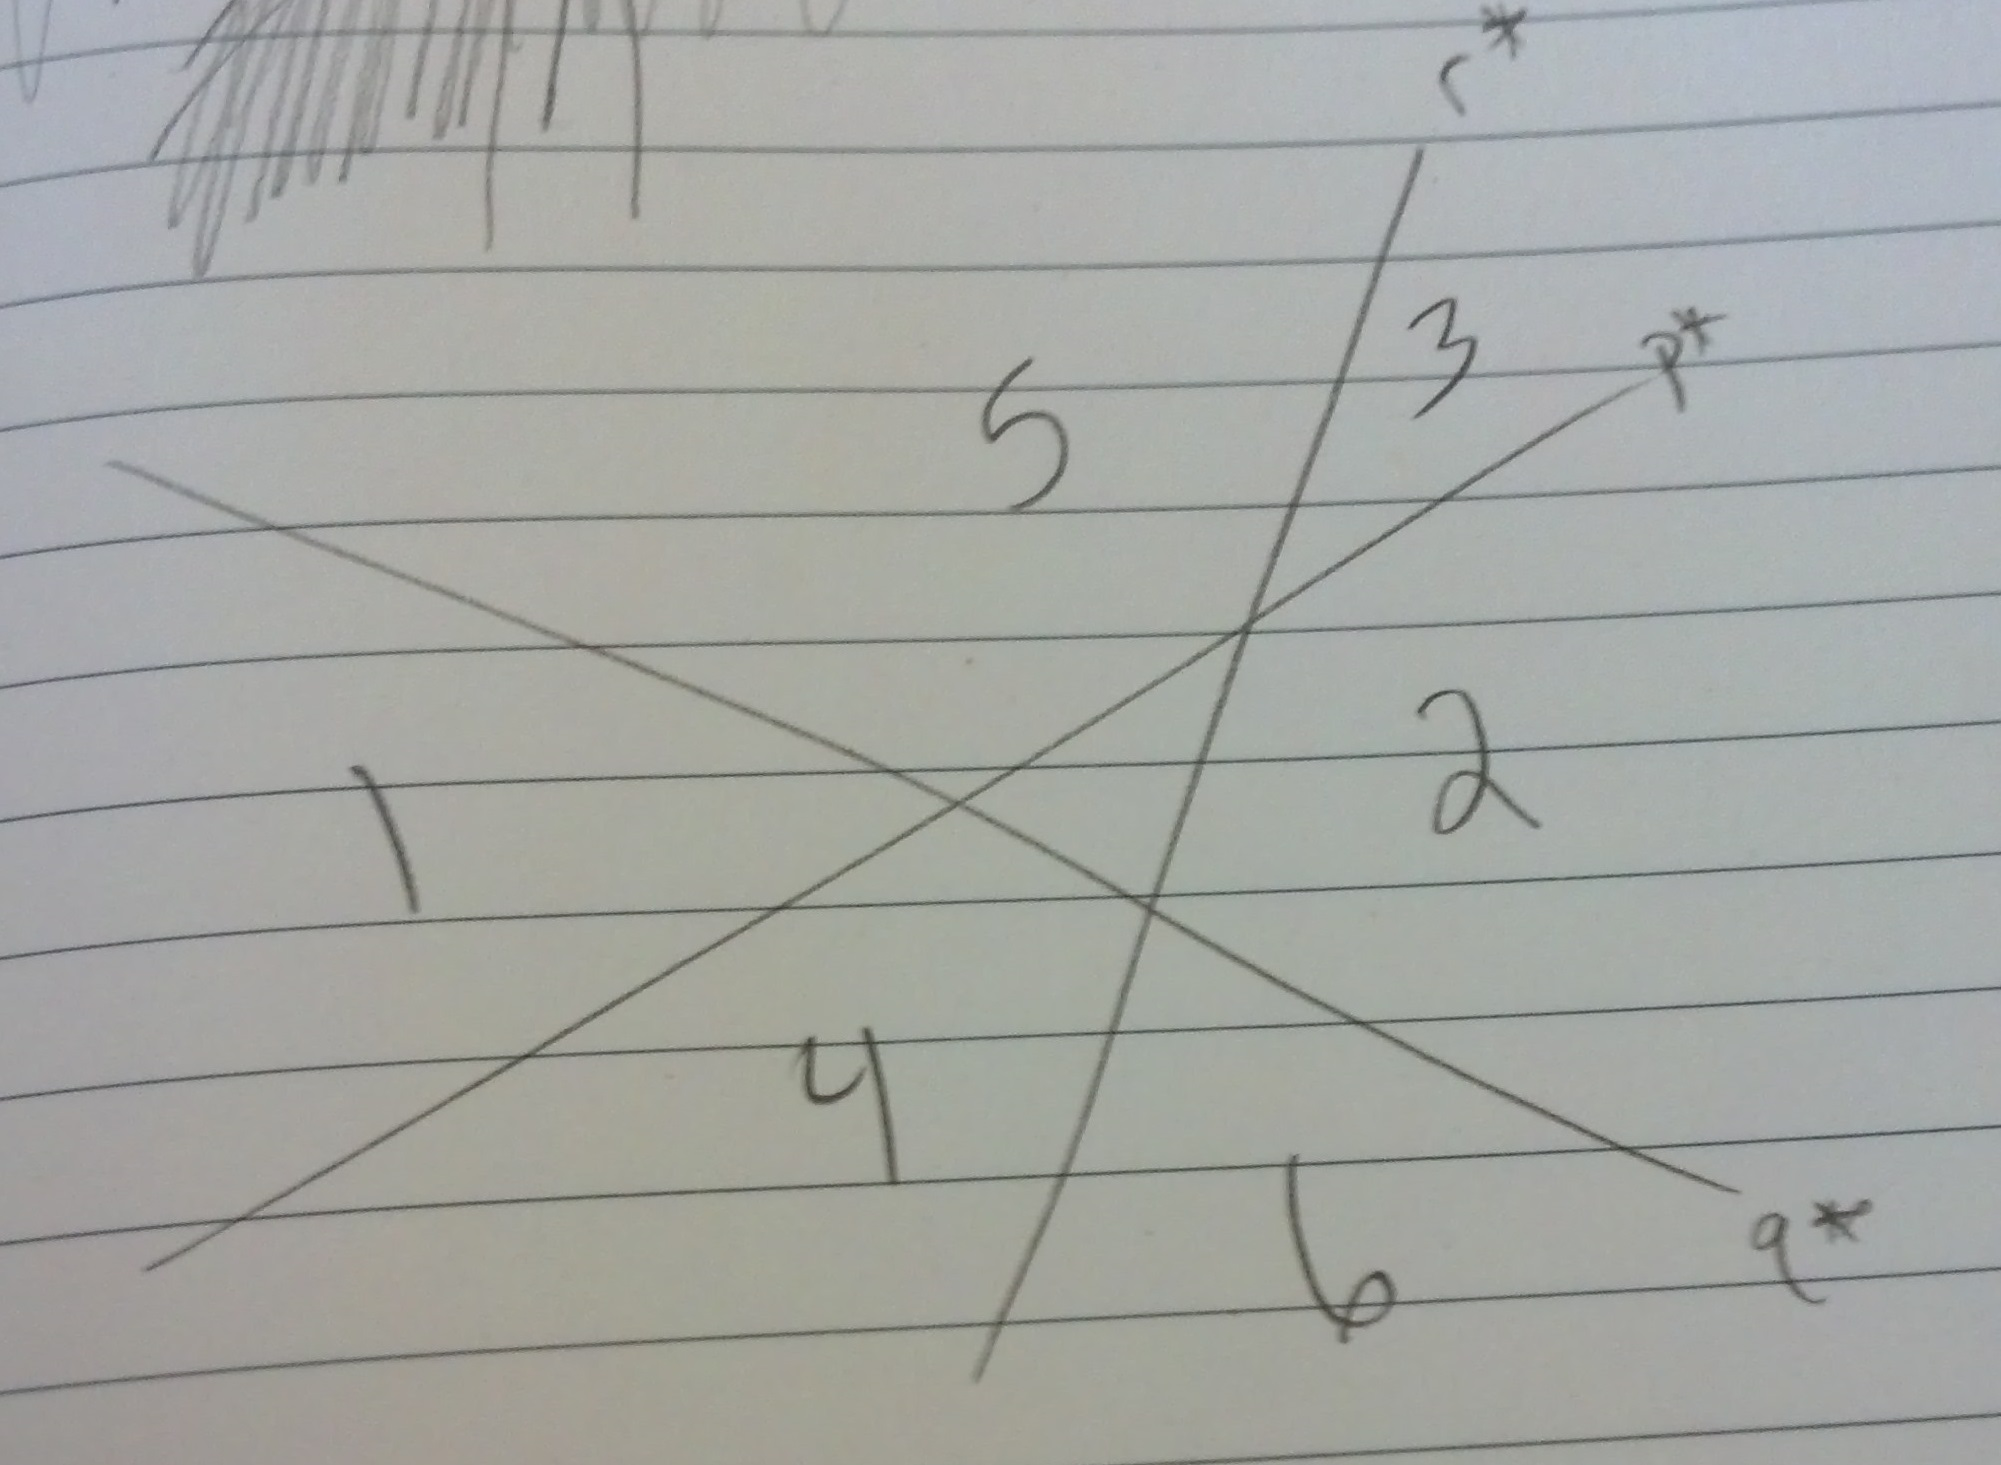
\includegraphics[height=4in]{cs266dual.jpg}
\caption{Illustration of the wedges}
\end{figure}

\subsection*{Problem 8.2b}

A line segment with negative slope with dualize to a top-bottom double wedge. This is because the x-coordinate is decreasing, meaning that the slope is decreasing so the wedge will appear in top-bottom order. 

\begin{figure}[H]
\centering
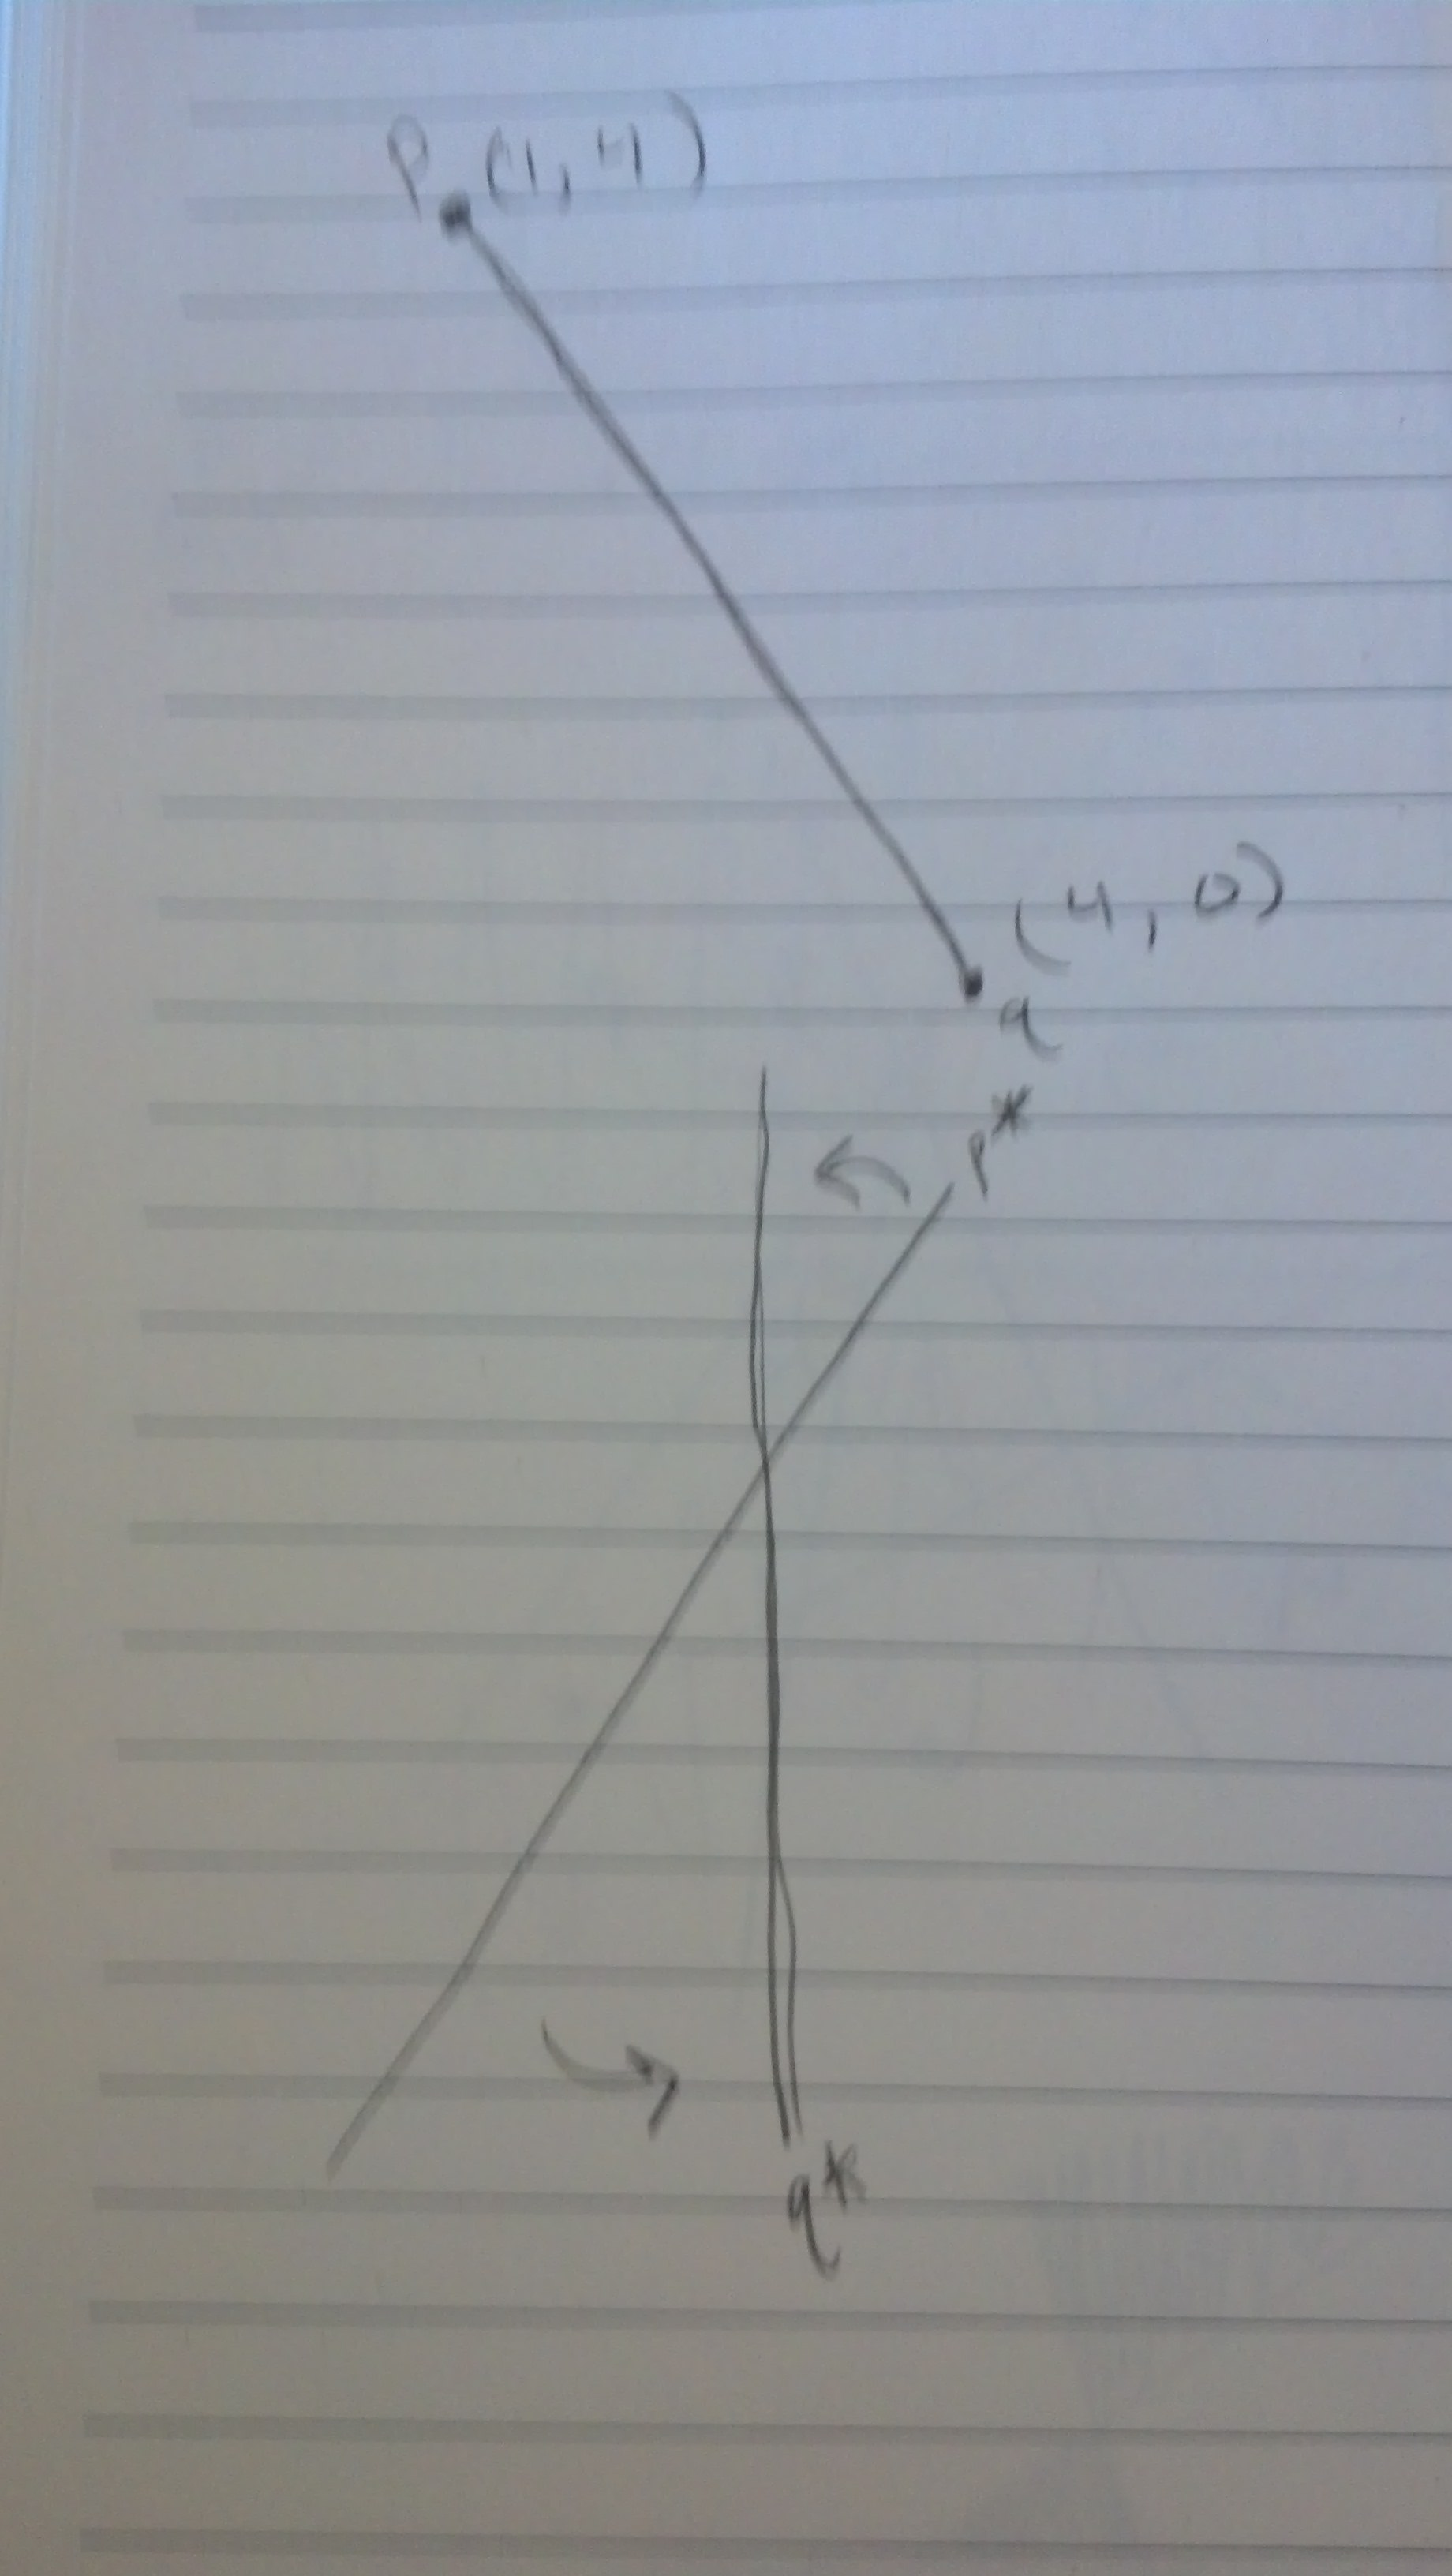
\includegraphics[height=4in]{cs266dual2.jpg}
\caption{Illustration of the wedges}
\end{figure}

\section*{Problem 8.6}

The duality transform is incidence-preserving thus the dual of the problem is whether any of the m points in the dual of L lie on any of the n lines in the dual of S. 


\end{document}








